\documentclass{article}

\newcounter{results}
\newcounter{questions}

\def\neg{{\sim}}
\def\Z{\mathbb{Z}}
\def\N{\mathbb{N}}
\def\R{\mathbb{R}}
\def\Q{\mathbb{Q}}
\def\E{\mathbb{E}}
\def\qed{\(\blacksquare\)}
\newcommand{\result}[1]{\stepcounter{results}{\bfseries Result \arabic{results}}: #1}
\newcommand{\question}[1]{\stepcounter{questions}{\bf \arabic{questions}}: #1}
\newenvironment{proof}[2][Proof]{\result{#2}\begin{trivlist} 
    \item[\hskip \labelsep {\sc #1:}]}{\qed\end{trivlist}}
\usepackage{array}
\usepackage{amsmath}
\usepackage{amssymb}
\usepackage{mathtools}
\usepackage{textcomp}
\usepackage{gensymb}
\usepackage{graphicx}
\usepackage{float}
\usepackage{caption}
\usepackage{amsfonts}
\usepackage[margin=1in]{geometry}

\renewcommand{\O}{\(\Omega\)}

\title{Lab 2 Progress Report}
\author{Ryan Coyne \\ Partner: Daniel Albu}

\begin{document}

\maketitle

\section{Introduction}
In this lab, we familiarized ourselves with using the Raspberry Pi, such as how to use SSH to access it from a laptop and how to write Python scripts that interact with the GPIO.

\section{Interacting with the Raspberry Pi}
To begin with, we learned to use SSH to remotely access the RPi. Next, we familiarized ourselves with the terminal including navigating the file system and editing text documents with nano and vim. We checked for software updates and made sure that the date and time were accurate. 

\section{Editing Text}
In the next part of the lab, we created a directory in our home directory called "notes" and created a file called "notes1.txt". We then used SCP on our personal computers to retrieve that file from the RPi and send it back. This was somewhat of a challenge because we didn't realize that on the school network, we are not able to access our laptops from the RPi over SSH so we needed to use our laptops to run the command and pull the file from the RPi. However, we did eventually get this to work. 

\section{Blinking a Built-in LED}
The Raspberry Pi has several general-purpose input/output pins, also known as GPIO pins. These can be used for a variety of input and output purposes. In this lab, we used these pins to control an LED using bash and Python. To begin with, we used terminal commands such as, \[\text{sudo sh -c 'echo "1" \(>\) /sys/class/leds/ACT/brightness'}\] to make calls to drivers on the RPi. This command turns the LED on. We also wrote a bash script that uses terminal commands to make the LED turn on for a half second and then turn it back off. 

\section{Using the GPIO from the Command Line}
Next, we connected the GPIO to a breadboard and created a simple circuit with an LED in series with a resistor (Figure 1). We then used a combination of terminal commands to select the GPIO port, set its mode to output, and then send a signal through that port to turn on the LED.

\begin{figure}[h!]
    \centering
    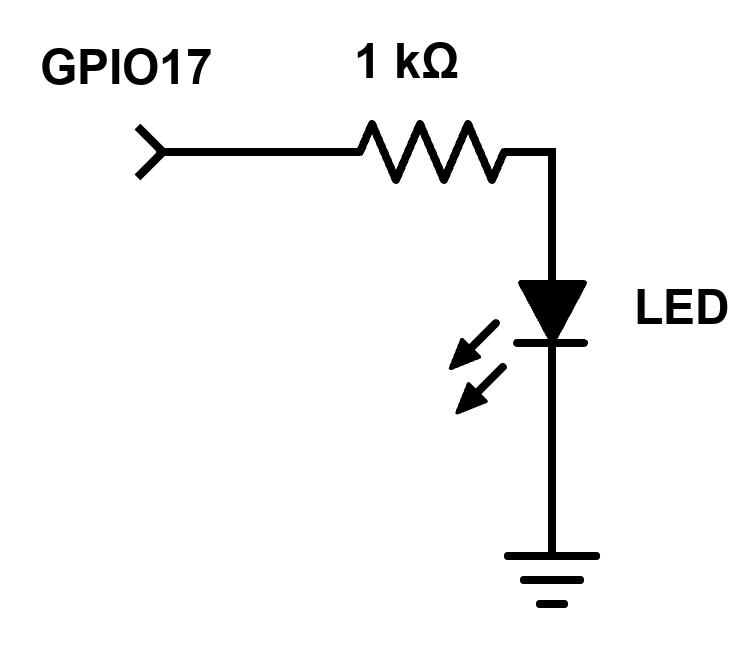
\includegraphics[width=0.4\linewidth]{simple_led.png}
    \caption{Simple LED Circuit}
\end{figure}

We also involved a switch. We created another circuit in which GPIO pin 16 would receive a signal when a switch was closed (Figure 2). To read the value of the switch we used the command \[\text{cat /sys/class/gpio/gpio16/value}\] in the terminal.

\begin{figure}[h!]
    \centering
    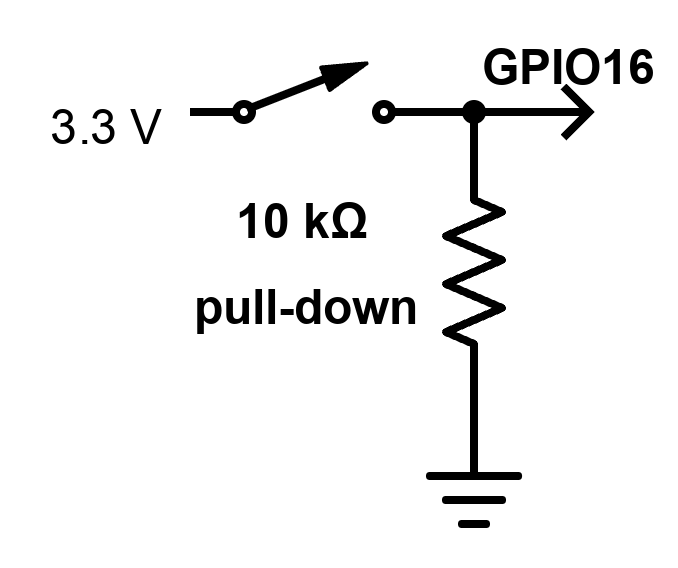
\includegraphics[width=0.4\linewidth]{simple_switch.png}
    \caption{Simple LED Circuit}
\end{figure}


\section{Using the GPIO with Python}
We next used Python to interface with the GPIO. We wrote a Python script that would allow the RPi to monitor the circuit in Figure 2, and when the switch is depressed, it would wait one second and then turn the LED on for two seconds. We also created a function that would increase the power sent to the led by 10\% each time the switch was pressed except if it was at 100\% power it would reset to 0\% the next time the switch was pressed. We also created a script that would blink "daniel albu" in Morse code on the LED. All of these scripts are in Lab2.py.

\section{What I Learned}
\begin{itemize}
    \item We have to use SCP on my laptop to pull files from the RPi because of the UNH network's DNS settings.
    \item I learned how to interface with the GPIO pins of the RPi with bash and Python. 
    \item I learned how to parse command line arguments with Python. This wasn't strictly necessary for the lab but it was convenient and easy to do. 
    \item I helped Ryan and Audrey get their switch working. 
\end{itemize}

\end{document}